\documentclass[aspectratio=169, 10pt]{beamer}

\usetheme{default}

\title[Stat. Comp. Bioinf \& SocNets.]{Statistical and computational methods for bioinformatics and social network analysis\linebreak{\small or how did I learn to stop worrying and love the bomb}}
\author[GGVY]{George G Vega Yon}
\institute[USC-PREVMED]{University of Southern California, Department of Preventive Medicine}

% Naigation
\setbeamertemplate{navigation symbols}{%
    \usebeamerfont{footline}%
    \usebeamercolor[fg]{footline}%
    \hspace{1em}%
    \insertframenumber/\inserttotalframenumber
}

% Some definitions
\def\cursection{\frame{\tableofcontents[current]}}
\newcommand{\ergmitopkg}[0]{\texttt{ergmito}}
\newcommand{\aphylopkg}[0]{\texttt{aphylo}}
\graphicspath{{.}{fig/}}

% Some important packages
\usepackage{apacite}
\hypersetup{colorlinks=true, allcolors=purple}
\usepackage{booktabs}
\linespread{1.3}
\usepackage{tabularx}

\usepackage{Sweave}
\begin{document}
\Sconcordance{concordance:slides.tex:slides.Rnw:%
1 432 1 49 0 10 1 2 0 393 1}


% ------------------------------------------------------------------------------
\begin{frame}[noframenumbering]
\maketitle
\end{frame}

% ------------------------------------------------------------------------------
\section{Paper 1: Exponential Random Graph Models for Small Networks}
\cursection

\begin{frame}
\frametitle{What are Exponential Random Graph Models}

Exponential Family Random Graph Models, aka ERGMs are:\pause

\begin{itemize}
\item Statistical models of (social) networks\pause
\item In simple terms: statistical inference on what network patterns/structures/motifs
govern the data-generating process
\begin{figure}
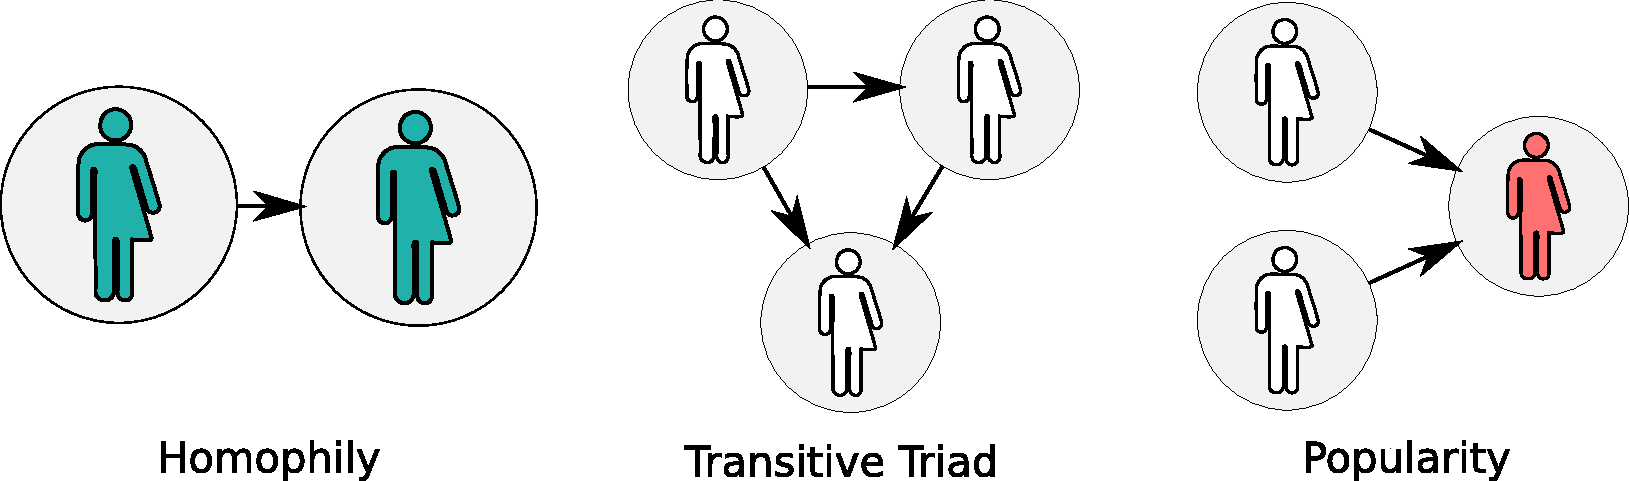
\includegraphics[width=.6\linewidth]{friendly-terms.pdf}
\end{figure}
\end{itemize}



\end{frame}


% ------------------------------------------------------------------------------
\begin{frame}
\def\fig1width{.45\linewidth}
\begin{figure}[tb]
\centering
\begin{tabular}{m{.2\linewidth}<\centering m{.4\linewidth}<\raggedright}
\toprule Representation & Description  \\ \midrule
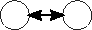
\includegraphics[width=\fig1width]{ergm-terms/mutual.pdf} & Mutual Ties (Reciprocity)\linebreak[4]$\sum_{i\neq j}y_{ij}y_{ji}$  \\
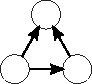
\includegraphics[width=\fig1width]{ergm-terms/ttriad.pdf} & Transitive Triad (Balance)\linebreak[4]$\sum_{i\neq j\neq k}y_{ij}y_{jk}y_{ik}$  \\

\includegraphics[width=\fig1width]{ergm-terms/homophily.pdf} & Homophily\linebreak[4]$\sum_{i\neq j}y_{ij}\mathbf{1}\left(x_i=x_j\right)$ \\
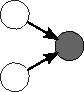
\includegraphics[width=\fig1width]{ergm-terms/nodeicov.pdf} & Covariate Effect for Incoming Ties\linebreak[4]$\sum_{i\neq j}y_{ij}x_j$ \\
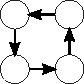
\includegraphics[width=\fig1width]{ergm-terms/fourcycle.pdf} & Four Cycle\linebreak[4]$\sum_{i\neq j \neq k \neq l}y_{ij}y_{jk}y_{kl}y_{li}$  \\
\bottomrule
\end{tabular}
\caption{\label{fig:ergm-structs}Besides of the common edge count statistic (number of ties in a graph), ERGMs allow measuring other more complex structures that can be captured as sufficient statistics. }
\end{figure}
\end{frame}

% ------------------------------------------------------------------------------
\begin{frame}
\frametitle{What are Exponential Random Graph Models: State of the Art}
\pause
Small-large (dozens to a couple of thousand vertices) networks

\begin{itemize}
\item Markov Chain Monte Carlo (MCMC) based approaches like MC-MLE or Robbins-Monro Stochastic approximation.
\item Maximum Pseudo Likelihood (MPLE)
\end{itemize}\pause

large-huge networks (up to the millions of vertices)

\begin{itemize}
\item Semi-parametric bootstrap
\item Conditional joint estimation (like snowball sampling, a.k.a. divide and conquer)
\item Equilibrium Expectation Algorithm (millions of vertices)
\end{itemize}\pause

But who cares about tiny to small networks?

\end{frame}

% ------------------------------------------------------------------------------
\begin{frame}
\frametitle{What are Exponential Random Graph Models: The MC-MLE approach}

One of the most popular methods for estimating ERGMs is the MC-MLE approach (citations here)

This consists on the folling steps

\begin{enumerate}
\item Start from a sensible guess on what should be the population parameters
(usually done using pseudo-MLE esimtation)
\item While the algorithm doesn't converge, do:
  \begin{enumerate}
  \item Simulate a stream of networks with the current state of the parameter,
  $\theta_t$
  \item Using the law of large numbers, approximate the ratio of likelihoods 
  based on the parameter $\theta_t$, this is the objective function
  \item Update the parameter by a Newton-Raphson step
  \item Next iteration
  \end{enumerate}
\end{enumerate}

\end{frame}

\begin{frame}
\frametitle{What are Exponential Random Graph Models: The MC-MLE approach}

MC-MLE works great (we have some simulations showing this), but it has some
problems:

\begin{itemize}
\item While lots of advances have been made, there are restrictions on what can
be done with it, after all, it is an approximation,
\item In the case of small networks, issues regarding near-degeneracy during
estimation are common (unstable MCMC process, bad sampling, problems)
\end{itemize}

What shall we do then?

\end{frame}

% ------------------------------------------------------------------------------
\begin{frame}
\frametitle{Exponential Random Graph Models for Small Networks}

\begin{itemize}
\item In the case of small-enough networks, computation of the likelihood becomes
computationally feasible\footnote{A thing mentioned in literature several times, although not much attention paid}
\item In the case of networks with 5 nodes, 1,048,576
different configurations, we can compute the likelihood exactly.
\end{itemize}

Using the exact likelihood opens a huge window of methodological-possibilities
\end{frame}

% ------------------------------------------------------------------------------
\begin{frame}
\frametitle{The \ergmitopkg{}}



\end{frame}

% ------------------------------------------------------------------------------
\begin{frame}
\frametitle{Paper 1 Simulation Studies}

In order to compare the MLE with the MC-MLE estimation method, we performed a simulation study with the following features:

\begin{itemize}
\item Draw 20,000 samples of groups of small networks
\item Each group had prescribed: (model parameters, number of networks, sizes of the networks)
\item We estimated the models using the ergm and ergmito R packages
\end{itemize}

\end{frame}

% ------------------------------------------------------------------------------
\begin{frame}
\frametitle{Paper 1 Simulation Studies: Error rate}

\begin{figure}
\centering
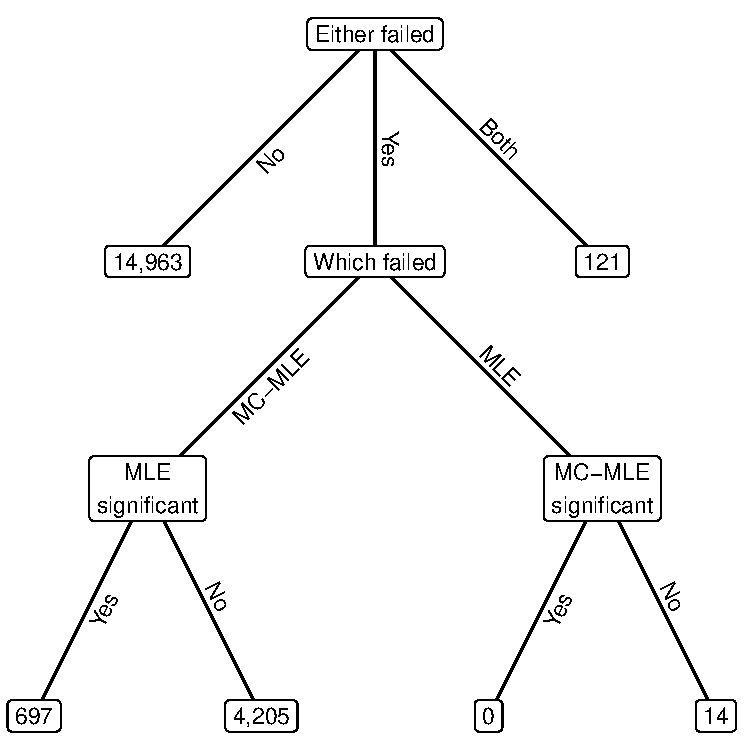
\includegraphics[width=.5\linewidth]{failed-tree.pdf}
\end{figure}

\end{frame}

% ------------------------------------------------------------------------------
\begin{frame}
\frametitle{Paper 1 Simulation Studies: Empirical Bias}

\begin{figure}
\centering
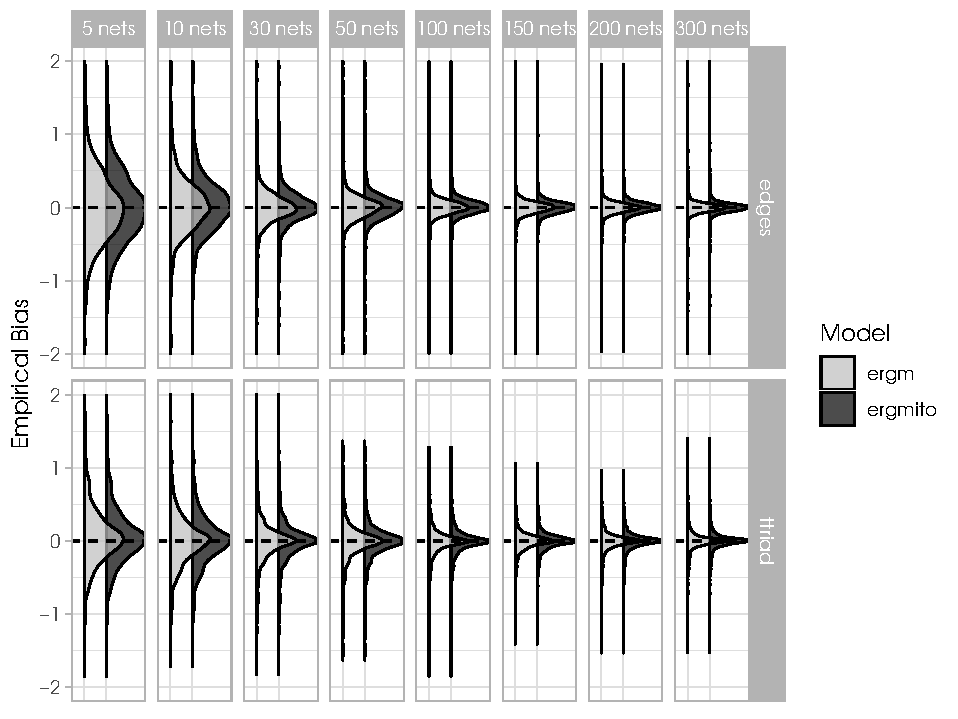
\includegraphics[width=.7\linewidth]{bias-02-various-sizes-4-5-ttriad.pdf}
\end{figure}

\end{frame}

% ------------------------------------------------------------------------------
\begin{frame}
\frametitle{Paper 1 Simulation Studies: Empirical Type I error}

\begin{table}[ht]
	\centering
	\begin{tabular}{ccccc}
		\toprule & & \multicolumn{2}{c}{P(Type I error)} \\ \cmidrule(r){3-4}
		Sample size & N. Simulations & MC-MLE & MLE & chi2 \\ 
		\midrule
		5 & 2,189 & 0.084 & 0.057 & 11.71 *** \\ 
		10 & 2,330 & 0.070 & 0.045 & 12.46 *** \\ 
		15 & 2,395 & 0.084 & 0.066 & 5.55 * \\ 
		20 & 2,430 & 0.074 & 0.060 & 3.58  \\ 
		30 & 2,460 & 0.057 & 0.052 & 0.67  \\ 
		50 & 2,495 & 0.046 & 0.044 & 0.17  \\ 
		100 & 2,499 & 0.048 & 0.048 & 0.00  \\ 
		\bottomrule
	\end{tabular}
	\caption{\label{tab:typeI}Empirical Type I error rates. The $\chi^2$ statistic is from a 2-sample test for equality of proportions, and the significance levels are given by *** $p < 0.001$, ** $p < 0.01$, and * $p < 0.05$. The lack of fitted samples in some levels is due to failure of the estimation method.} 
\end{table}

\end{frame}

% ------------------------------------------------------------------------------
\begin{frame}
\frametitle{Paper 1 Simulation Studies: Elapsed time}

\begin{figure}
\centering
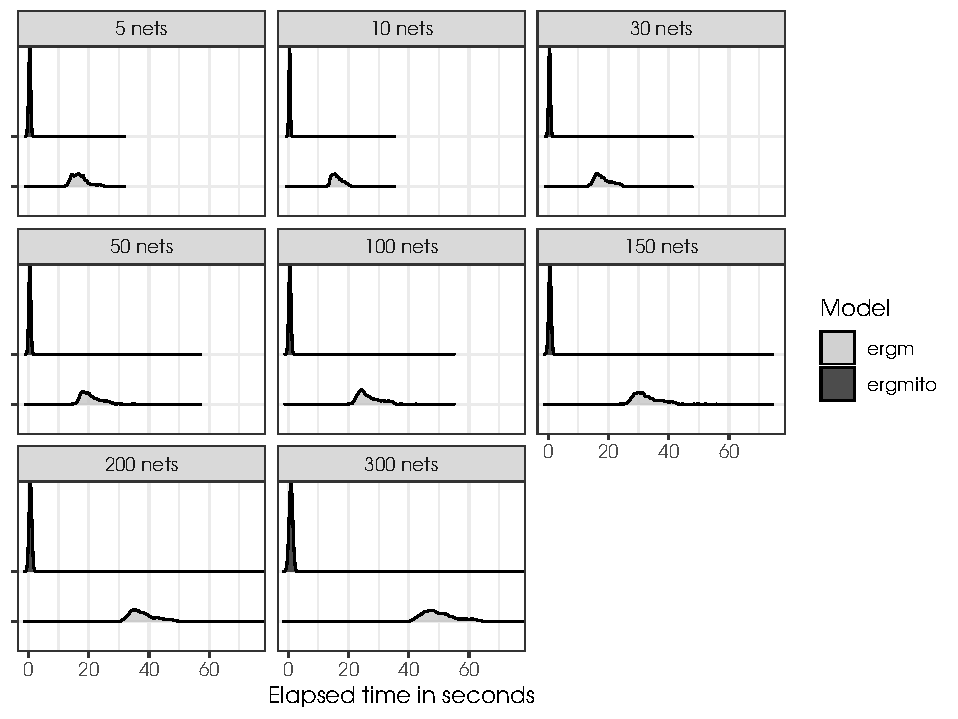
\includegraphics[width=.7\linewidth]{bias-elapsed-02-various-sizes-4-5-ttriad.pdf}
\end{figure}

\end{frame}

% ------------------------------------------------------------------------------
\section{Paper 2: On the prediction of gene functions using phylogenetic trees}
\cursection

\begin{frame}
\frametitle{Phylogenetic Trees}

\begin{itemize}
\item It can be very general: think of the tree of life
\item Nowadays, thanks to gene-sequencing techniques, we are building trees at the
gene level (using sequence-alignment methods, i.e. comparing gene sequences to see how much similar/different two genes are between and within species (whattt!)).
\item A single phylogenetic tree can host multiple species
\end{itemize}

\end{frame}

\begin{frame}
A common phylogenetic tree
\end{frame}

\begin{frame}
\frametitle{Gene Functional Annotations}

The Gene Ontology Project

\begin{table}
\small
\begin{tabular}{lm{.5\linewidth}}
\toprule
\textbf{Accession} & GO:0060047 \\
\textbf{Name} & heart contraction \\
\textbf{Ontology} & biological\_process \\
\textbf{Synonyms} & heart beating, cardiac contraction, hemolymph circulation \\
\textbf{Alternate} & IDs None \\
\textbf{Definition} & The multicellular organismal process in which the heart decreases in volume in a 
characteristic way to propel blood through the body. Source: GOC:dph \\
\bottomrule
\end{tabular}
\end{table}

source: http://amigo.geneontology.org/amigo/term/GO:0060047


\end{frame}

\begin{frame}
\frametitle{Speciation}
\begin{figure}
\centering
\def\svgwidth{.9\linewidth}
\tiny
% Source 
\input{fig/Drosophila_speciation_experiment.pdf_tex}
\caption{\citeA{Dodd1989}: After one year of isolation, flies showed a significant level or assortativity in mating (\href{https://commons.wikimedia.org/wiki/File:Drosophila_speciation_experiment.svg}{wikimedia})}
\end{figure}
\end{frame}

\begin{frame}
\frametitle{Duplication}
\begin{figure}
\centering
\def\svgwidth{.7\linewidth}
\tiny
% Source : https://en.wikipedia.org/wiki/File:Evolution_fate_duplicate_genes_-_vector.svg
\input{fig/Evolution_fate_duplicate_genes_-_vector.pdf_tex}
\caption{A key part of molecular innovation, gene duplication provides opportunity for new functions to emerge (\href{https://en.wikipedia.org/wiki/File:Evolution_fate_duplicate_genes_-_vector.svg}{wikimedia})}
\end{figure}
\end{frame}


\begin{frame}
\frametitle{An evolutionary model of gene functions}

The general points of the model
\begin{itemize}
\item The rootnode in a phylogenetic tree is the best idea we have about the past, meaning,
it could be that the tree has more behind, i.e. so functions may be gained since the beginning
\item At each step in evolution (interior node), there is a probability that the gene may
gain/loss the function
\item Those probabilities vary depending on the type of the node: We belive that functional
changes may happen at Duplication nodes
\item That's it!
\end{itemize}
\end{frame}

\begin{frame}
\frametitle{An evolutionary model of gene functions: Formal statement}

The whole is based on the markov-assumption: The current state of the gene can be
fully explained by its parent(s).

For this we use Felsensteins' pruning algorithm (also known as...)

Formally

$$
P(x = 1) = P(x = 1| x_p = 0)P(\mbox{Gain}) + P(x = 1| x_p = 1)P(\mbox{No loss})
$$

\end{frame}

\begin{frame}
\frametitle{The \aphylopkg{}}
\end{frame}


% ------------------------------------------------------------------------------
\section{Future directions}
\begin{frame}
\frametitle{Future directions: ERGMitos}

\begin{itemize}
\item Identify an adequate test for goodness-of-fit assesment
\item Extend to estimation of large graphs by splitting the networks in induced-subgraphs
\end{itemize}

\end{frame}

\begin{frame}
\frametitle{Future directions: Gene functional prediction}

Possible venues to continue

\begin{itemize}
\item Incorporate more external information using leaf(and node?) level features.
\item Adapt the model to incorporate joint estimation of functions using pseudo-likelihood.

$$
P(a, b, c) \approx P(a,b)P(b,c)P(a,c)
$$
\item Make the model hierarchical when pooling trees: different mutation rates.
\end{itemize}

\end{frame}


% ------------------------------------------------------------------------------
\section{Things that are very interesting but I most probably won't have any time to discuss with the attendees}

\begin{frame}
Here are some by-products of my research here at USC

\begin{itemize}
\item The slurmR R package
\item The pruner C++ library
\item The fmcmc R package
\end{itemize}

\end{frame}

\begin{frame}[allowframebreaks]
\frametitle{References}
\bibliographystyle{apacite}
\bibliography{bibliography.bib}
\end{frame}

\end{document}

